\chapter{Sicurezza dei Sistemi Operativi}
Un SO (Sistema Operativo), o OS (Operating System), gestisce il modo in cui le applicazioni software accedono alle risorse hardware del calcolatore:
\begin{itemize} 
  \item CPU
  \item Memoria principale
  \item Memoria secondaria
  \item Periferiche di I/O
  \item Interfacce di rete
\end{itemize}
Un OS fornisce un’interfaccia semplificata e consistente a utenti e applicazioni al fine di interagire con i componenti hardware. Grazie a questa astrazione è possibile sviluppare programmi software senza preoccuparsi della particolare tipologia di hardware sul quale saranno eseguiti. Grazie a questa astrazione è possibile sviluppare programmi software senza preoccuparsi della particolare tipologia di hardware sul quale saranno eseguiti. Gli OS svolgono numerose funzioni, alcune delle quali strettamente legate a problemi di sicurezza, in particolare vedremo:
\begin{itemize} 
  \item meccanismi di autenticazione
  \item sicurezza dei processi
  \item sicurezza del filesystem
  \item sicurezza della memoria
\end{itemize}
\section{Meccanismi di Autenticazione}
Un OS deve poter identificare i propri utenti in modo sicuro, i.e. utenti diversi potrebbero avere permessi di accesso alle risorse diversi. Un meccanismo di autenticazione standard ampiamente usato consiste nell’inserimento di un username e di una password: se la password inserita coincide con la password memorizzata dall'OS per il dato username allora l'utente viene autenticato. Un OS deve dunque memorizzare la password di ogni utente che può accedere al sistema. Generalmente gli OS memorizzano le password criptate attraverso funzioni hash in un file o in un apposito database. Grazie alla proprietà one-way delle funzioni hash, un attaccante che riesce ad accedere al file dove sono memorizzate le password non può ricostruire facilmente il loro valore. Tali file si trovano:
\begin{itemize} 
  \item per Windows in system32 - config - SAM
  \item per Linux in $/etc/passwd$ e in $/etc/shadow$ (solo l’utente root può leggerle)
\end{itemize}

\subsection{Possibili attacchi}
\begin{itemize} 
  \item \textbf{Brute Force}: attacco offline, tutte le possibili password per un dato alfabeto vengono generate automaticamente, criptate con la funzione hash usata dal sistema di autenticazione e confrontate con le password memorizzate
  \item \textbf{Dizionario}: attacco offline, liste di parole comuni (es: nomi) che vengono criptate con la funzione hash usata dal sistema di autenticazione e confrontate con le password memorizzate
  \item \textbf{Rainbow tables}
\end{itemize}
\subsection{Password Robuste}
Per la definizione di password robuste a tali attacchi vanno seguite delle ben definite linee guida:
\begin{itemize}
  \item evitare parole comuni (e.g.: nomi)
  \item evitare password brevi
  \item usare caratteri maiuscoli E minuscoli
  \item usare caratteri speciali
  \item usare i numeri
\end{itemize}
Un esempio di password robusta è: "Voglio compr@re 11 Cani!": per scoprire questa password con un attacco brute-force in 60 giorni dovrei disporre di un computer in grado di generare circa $3,86 x 10^{44} PW/sec$. Per rendere la struttura ancora più sicura si può impostare una scadenza alla password.
\subsection{Password Salt}
Il \textbf{Salt} consiste nell'aggiunta di bit random all'input di una funzione hash (o di un algoritmo di crittografia) al fine di aumentare la randomicità dell'output. Nel caso dell’autenticazione è possibile associare un numero random all'userID dell’utente, seguendo la forma: \newline \newline
\textbf{salt = numero random + userID} \newline \newline
\begin{figure}[htbp]
	\centering%
	\subfigure%
	{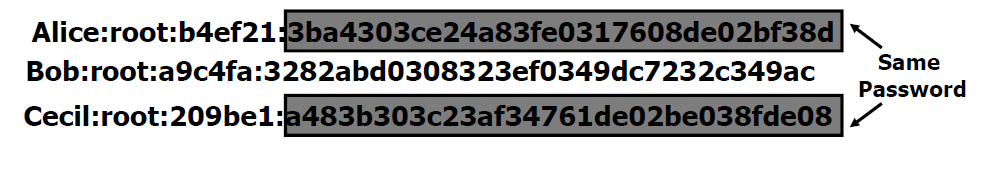
\includegraphics[height=8cm, width=13cm, keepaspectratio]{Immagini/Capitolo9/password.png}}
	\caption{Esempi di Salt \label{fig:salt}} 	
\end{figure}
\newpage
Il processo di autenticazione funziona nel seguente modo:
\begin{itemize}
  \item L’utente inserisce il suo userID X e la password P
  \item Il processo di autenticazione dell’OS recupera il salt S per l’userID X e l’hash H del salt concatenato alla password associata a X
  \item OS verifica se $HASH(S \vert \vert P) == H$
\end{itemize}
\begin{figure}[htbp]
	\centering%
	\subfigure%
	{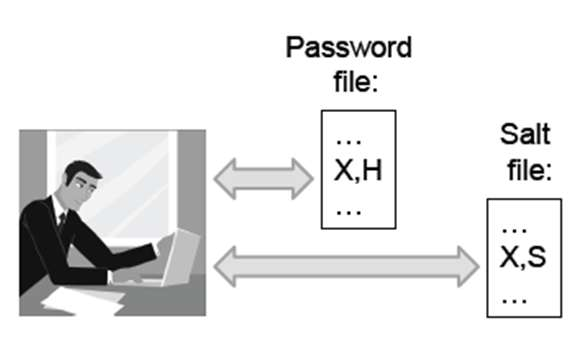
\includegraphics[height=8cm, width=8cm, keepaspectratio]{Immagini/Capitolo9/password2.png}}
	\caption{Processo di autenticazione con Salt \label{fig:salt}} 	
\end{figure}
Tale meccanismo comporta evidenti benefici. Se l’attaccante non può trovare il salt associato con l’userID, allora lo spazio di ricerca per un attacco con dizionario cresce notevolmente, diventando $2^{B} x D$, dove B è il numero di bit del Salt, mentre D lo spazio del dizionario. \newline
Inoltre, anche se l'attaccante fosse in grado di recuperare il salt memorizzato in forma criptata dall’OS, questo meccanismo consente di rallentare notevolmente l’attacco con dizionario, rendendolo valido per un userID alla volta. Senza salt è possibile crackare molte password nello stesso momento, in quanto si ha solo bisogno dell'hash di ogni possibile password e di confrontarlo con tutti gli hash memorizzati. Con il meccanismo di salt, invece, ogni possibile password va
concatenata al salt ad essa associato prima di calcolarne l'hash.